% answers.tex —— 2013 年全国Ⅰ卷（文科） · 参考答案与详细解析片段
% 由 tools/generate_projects.py 依来源总账自 2013/2013_数学真题_全国1文_试题.md + 2013/2013_数学真题_全国1文_解析正文.md + 2013/2013_数学真题_全国1文_答案要点.md 生成，勿手改（改源 MD 后重跑）


\begin{gktip}
固定源 PDF 是印刷页码 827–828 的两页题面，不附答案或解析。以下各题均依据题面独立复算，\textbf{非官方标准答案}；第 7、9、11、18、19、22 题图形在 LaTeX 工程中以 TikZ/PGFPlots 矢量源重绘。
\end{gktip}

\gkpart{一、选择题}

\begin{answer}
\gksolhead{1}{}

\textbf{题目}：

已知集合 $A=\{1,2,3,4\}$，$B=\{x\mid x=n^2,\ n\in A\}$，则 $A\cap B=$\mbox{（　　）}

（A）$\{1,4\}$　　（B）$\{2,3\}$　　（C）$\{9,16\}$　　（D）$\{1,2\}$

\Needspace{4\baselineskip}
\textbf{解析}

$B=\{1,4,9,16\}$，与 $A$ 取交集即得 $\{1,4\}$，选 A。

\gkanswer{答案：A}

\end{answer}
\begin{answer}
\gksolhead{2}{}

\textbf{题目}：

$\dfrac{1+2i}{(1-i)^2}=$\mbox{（　　）}

（A）$-1-\dfrac12i$　　（B）$-1+\dfrac12i$　　（C）$1+\dfrac12i$　　（D）$1-\dfrac12i$

\Needspace{4\baselineskip}
\textbf{解析}

\Needspace{5\baselineskip}
$(1-i)^2=-2i$，所以

\nopagebreak[4]
\[
\frac{1+2i}{(1-i)^2}=\frac{1+2i}{-2i}=1-\frac12i,
\]

选 D。

\gkanswer{答案：D}

\end{answer}
\begin{answer}
\gksolhead{3}{}

\textbf{题目}：

从 $1,2,3,4$ 中任取 $2$ 个不同的数，则取出的 $2$ 个数之差的绝对值为 $2$ 的概率是\mbox{（　　）}

（A）$\dfrac12$　　（B）$\dfrac13$　　（C）$\dfrac14$　　（D）$\dfrac16$

\Needspace{4\baselineskip}
\textbf{解析}

从四个数中取两个共有 $\binom42=6$ 种等可能结果；差的绝对值为 $2$ 的只有 $\{1,3\}$、$\{2,4\}$ 两种，概率为 $2/6=1/3$，选 B。

\gkanswer{答案：B}

\end{answer}
\begin{answer}
\gksolhead{4}{}

\textbf{题目}：

已知双曲线 $C:\dfrac{x^2}{a^2}-\dfrac{y^2}{b^2}=1\ (a>0,b>0)$ 的离心率为 $\dfrac{\sqrt5}{2}$，则 $C$ 的渐近线方程为\mbox{（　　）}

（A）$y=\pm\dfrac14x$　　（B）$y=\pm\dfrac13x$　　（C）$y=\pm\dfrac12x$　　（D）$y=\pm x$

\Needspace{4\baselineskip}
\textbf{解析}

$e^2=1+b^2/a^2=5/4$，故 $b/a=1/2$。渐近线为 $y=\pm(b/a)x=\pm x/2$，选 C。

\gkanswer{答案：C}

\end{answer}
\begin{answer}
\gksolhead{5}{}

\textbf{题目}：

已知命题 $p:\forall x\in\mathbb R,\ 2^x<3^x$；命题 $q:\exists x\in\mathbb R,\ x^3=1-x^2$，则下列命题中为真命题的是\mbox{（　　）}

（A）$p\land q$　　（B）$\neg p\land q$　　（C）$p\land\neg q$　　（D）$\neg p\land\neg q$

\Needspace{4\baselineskip}
\textbf{解析}

当 $x<0$ 时 $2^x>3^x$，故 $p$ 为假。函数 $x^3+x^2-1$ 连续，且在 $0,1$ 处函数值异号，故存在实根，$q$ 为真；选 B。

\gkanswer{答案：B}

\end{answer}
\begin{answer}
\gksolhead{6}{}

\textbf{题目}：

设首项为 $1$，公比为 $\dfrac23$ 的等比数列 $\{a_n\}$ 的前 $n$ 项和为 $S_n$，则\mbox{（　　）}

（A）$S_n=2a_n-1$　　（B）$S_n=3a_n-2$　　（C）$S_n=4-3a_n$　　（D）$S_n=3-2a_n$

\Needspace{4\baselineskip}
\textbf{解析}

\Needspace{5\baselineskip}
等比求和得

\nopagebreak[4]
\[
S_n=\frac{1-(2/3)^n}{1-2/3}=3-2a_n,
\]

选 D。

\gkanswer{答案：D}

\end{answer}
\begin{answer}
\gksolhead{7}{}

\textbf{题目}：

执行下面的程序框图，若输入的 $t\in[-1,3]$，则输出的 $s$ 属于\mbox{（　　）}
\nopagebreak[4]
\begin{center}% 2013 全国卷Ⅰ文科第 7 题：分段计算程序框图。
\begin{tikzpicture}[font=\footnotesize, >=Stealth, node distance=4mm, line width=0.4pt,
  box/.style={draw, minimum height=1.65em, minimum width=6.3em, inner xsep=5pt},
  term/.style={draw, rounded corners=6pt, minimum height=1.65em, inner xsep=8pt},
  io/.style={draw, trapezium, trapezium left angle=70, trapezium right angle=110,
             minimum height=1.65em, inner xsep=4pt},
  dec/.style={draw, diamond, aspect=2.25, inner sep=1.6pt}]
  \node[term] (start) {开始};
  \node[io, below=of start] (input) {输入 $t$};
  \node[dec, below=7mm of input] (cond) {$t<1$};
  \node[box, below left=8mm and 12mm of cond] (left) {$s=3t$};
  \node[box, below right=8mm and 12mm of cond] (right) {$s=4t-t^2$};
  \coordinate (join) at ($(left.south)!0.5!(right.south)+(0,-5mm)$);
  \node[io, below=8mm of join] (output) {输出 $s$};
  \node[term, below=of output] (end) {结束};
  \draw[->] (start) -- (input);
  \draw[->] (input) -- (cond);
  \draw[->] (cond.west) -| node[pos=0.22,above] {是} (left.north);
  \draw[->] (cond.east) -| node[pos=0.22,above] {否} (right.north);
  \draw[->] (left.south) |- (join);
  \draw[->] (right.south) |- (join);
  \draw[->] (join) -- (output);
  \draw[->] (output) -- (end);
\end{tikzpicture}
\end{center}
\nopagebreak[4]
（A）$[-3,4]$　　（B）$[-5,2]$　　（C）$[-4,3]$　　（D）$[-2,5]$

\Needspace{4\baselineskip}
\textbf{解析}

当 $-1\leqslant t<1$ 时，$s=3t\in[-3,3)$；当 $1\leqslant t\leqslant3$ 时，$s=4t-t^2$，其最大值为 $4$、最小值为 $3$。并集为 $[-3,4]$，选 A。

\gkanswer{答案：A}

\end{answer}
\begin{answer}
\gksolhead{8}{}

\textbf{题目}：

$O$ 为坐标原点，$F$ 为抛物线 $C:y^2=4\sqrt2x$ 的焦点，$P$ 为 $C$ 上一点，若 $|PF|=4\sqrt2$，则 $\triangle POF$ 的面积为\mbox{（　　）}

（A）$2$　　（B）$2\sqrt2$　　（C）$2\sqrt3$　　（D）$4$

\Needspace{4\baselineskip}
\textbf{解析}

\Needspace{5\baselineskip}
抛物线参数 $p=\sqrt2$，焦点为 $(\sqrt2,0)$。由 $PF=x+\sqrt2=4\sqrt2$ 得 $x=3\sqrt2$，再由方程得 $|y|=2\sqrt6$。故

\nopagebreak[4]
\[
S_{\triangle POF}=\frac12\cdot\sqrt2\cdot2\sqrt6=2\sqrt3,
\]

选 C。

\gkanswer{答案：C}

\end{answer}
\begin{answer}
\gksolhead{9}{}

\textbf{题目}：

函数 $f(x)=(1-\cos x)\sin x$ 在 $[-\pi,\pi]$ 的图象大致为\mbox{（　　）}
\nopagebreak[4]
\begin{center}% 2013 全国卷Ⅰ文科第 9 题：四个函数图象选项。
\begin{tikzpicture}[>=Stealth, scale=0.73, line width=0.42pt]
  \foreach \x/\y/\lab in {0/0/A,4.55/0/B,0/-3.35/C,4.55/-3.35/D} {
    \begin{scope}[shift={(\x,\y)}]
      \node[font=\scriptsize] at (-1.62,1.20) {$(\lab)$};
      \draw[->] (-1.55,0)--(1.72,0) node[right,font=\scriptsize] {$x$};
      \draw[->] (0,-1.16)--(0,1.30) node[above,font=\scriptsize] {$y$};
      \draw (0.08,0.08)--(-0.08,-0.08) node[below left,font=\scriptsize] {$O$};
      \draw (0,1.0)--(0.08,1.0) node[right,font=\scriptsize] {$1$};
      \node[below,font=\scriptsize] at (-1.45,0) {$-\pi$};
      \node[below,font=\scriptsize] at (1.45,0) {$\pi$};
    \end{scope}
  }
  % A
  \draw[thick] (-1.45,0) .. controls (-1.20,0.72) and (-0.78,0.98) .. (-0.42,0.50)
    .. controls (-0.18,0.18) and (-0.12,0.02) .. (0,0)
    .. controls (0.25,-0.10) and (0.58,-0.90) .. (1.05,-0.80)
    .. controls (1.29,-0.73) and (1.40,-0.27) .. (1.45,0);
  % B
  \draw[thick] (3.10,0) .. controls (3.37,-0.28) and (3.65,-0.12) .. (3.92,-0.05)
    .. controls (4.23,0.04) and (4.35,-0.18) .. (4.55,0)
    .. controls (4.79,0.12) and (5.02,1.06) .. (5.42,1.05)
    .. controls (5.88,1.03) and (6.04,0.13) .. (6.00,0);
  % C
  \draw[thick] (-1.45,-3.35) .. controls (-1.20,-4.13) and (-0.88,-4.45) .. (-0.52,-4.08)
    .. controls (-0.22,-3.76) and (-0.15,-3.42) .. (0,-3.35)
    .. controls (0.26,-3.21) and (0.58,-2.39) .. (1.02,-2.38)
    .. controls (1.31,-2.38) and (1.40,-3.08) .. (1.45,-3.35);
  % D
  \draw[thick] (3.10,-3.35) .. controls (3.40,-3.40) and (3.70,-4.46) .. (4.05,-4.38)
    .. controls (4.34,-4.31) and (4.37,-3.50) .. (4.55,-3.35)
    .. controls (4.77,-3.16) and (5.02,-2.37) .. (5.42,-2.39)
    .. controls (5.81,-2.41) and (5.95,-3.12) .. (6.00,-3.35);
\end{tikzpicture}
\end{center}
\nopagebreak[4]
\Needspace{4\baselineskip}
\textbf{解析}

$1-\cos x\geqslant0$，故函数在 $[-\pi,0]$ 上非正、在 $[0,\pi]$ 上非负；在 $-\pi,0,\pi$ 处为零，且原点附近与 $x^3/2$ 同号，故选 C。

\gkanswer{答案：C}

\end{answer}
\begin{answer}
\gksolhead{10}{}

\textbf{题目}：

已知锐角 $\triangle ABC$ 的内角 $A,B,C$ 的对边分别为 $a,b,c$，$23\cos^2A+\cos2A=0$，$a=7$，$c=6$，则 $b=$\mbox{（　　）}

（A）$10$　　（B）$9$　　（C）$8$　　（D）$5$

\Needspace{4\baselineskip}
\textbf{解析}

\Needspace{5\baselineskip}
由 $\cos2A=2\cos^2A-1$ 得 $\cos A=1/5$。再由余弦定理

\nopagebreak[4]
\[
\frac{b^2+6^2-7^2}{2\cdot b\cdot6}=\frac15,
\]

解得正根 $b=5$，选 D。

\gkanswer{答案：D}

\end{answer}
\begin{answer}
\gksolhead{11}{}

\textbf{题目}：

某几何体的三视图如图所示，则该几何体的体积为\mbox{（　　）}
\nopagebreak[4]
\begin{center}% 2013 全国卷Ⅰ文科第 11 题：三视图与尺寸标注。
\begin{tikzpicture}[font=\scriptsize, >=Stealth, line width=0.4pt]
  % 左上：半圆柱投影
  \begin{scope}
    \draw (0,2)--(4,2)--(4,0)--(0,0)--cycle;
    \draw (0,0) arc[start angle=180,end angle=360,radius=2];
    \draw[<->] (0,-0.42)--(4,-0.42) node[midway,below] {$4$};
    \draw[<->] (-0.35,0)--(-0.35,2) node[midway,left] {$2$};
  \end{scope}
  % 右上：侧视图阶梯
  \begin{scope}[xshift=5.65cm]
    \draw (0,0)--(4,0)--(4,1)--(2,1)--(2,4)--(0,4)--cycle;
    \draw[<->] (-0.35,0)--(-0.35,4) node[midway,left] {$4$};
    \draw[<->] (0,4.36)--(2,4.36) node[midway,above] {$2$};
    \draw[<->] (4.36,0)--(4.36,1) node[midway,right] {$2$};
  \end{scope}
  % 左下：俯视图
  \begin{scope}[yshift=-6.30cm]
    \draw (0,0)--(4,0)--(4,4)--(0,4)--cycle;
    \draw (0,2)--(4,2);
    \draw[<->] (-0.35,0)--(-0.35,4) node[midway,left] {$4$};
    \draw[<->] (4.36,0)--(4.36,2) node[midway,right] {$2$};
  \end{scope}
\end{tikzpicture}
\end{center}
\nopagebreak[4]
（A）$16+8\pi$　　（B）$8+8\pi$　　（C）$16+16\pi$　　（D）$8+16\pi$

\Needspace{4\baselineskip}
\textbf{解析}

三视图对应的立体可分为一个长方体和一个半圆柱：长方体体积为 $4\times2\times2=16$，半圆柱体积为 $\tfrac12\pi\cdot2^2\cdot4=8\pi$。故总体积为 $16+8\pi$，选 A。

\gkanswer{答案：A}

\end{answer}
\begin{answer}
\gksolhead{12}{}

\textbf{题目}：

\Needspace{5\baselineskip}
已知函数

\nopagebreak[4]
\[
f(x)=\begin{cases}
-x^2+2x,&x\leqslant0,\\
\ln(x+1),&x>0,
\end{cases}
\]

若 $|f(x)|\geqslant ax$，则 $a$ 的取值范围是\mbox{（　　）}

（A）$(-\infty,0]$　　（B）$(-\infty,1]$　　（C）$[-2,1]$　　（D）$[-2,0]$

\Needspace{4\baselineskip}
\textbf{解析}

\Needspace{5\baselineskip}
当 $x<0$ 时，$f(x)<0$，所以 $|f(x)|=x^2-2x$，不等式化为

\nopagebreak[4]
\[
x^2-(a+2)x=x\bigl[x-(a+2)\bigr]\geqslant0.
\]

\Needspace{5\baselineskip}
要对一切 $x<0$ 成立，须且只须 $a+2\geqslant0$，即 $a\geqslant-2$。在 $x=0$ 时不等式恒成立。对 $x>0$，须有

\nopagebreak[4]
\[
a\leqslant\frac{\ln(1+x)}x.
\]

右端在 $x\to+\infty$ 时趋于 $0$，且为正，故 $a\leqslant0$。合并得 $-2\leqslant a\leqslant0$，选 D。

\gkanswer{答案：D}

\end{answer}
\gkpart{二、填空题}

\begin{answer}
\gksolhead{13}{}

\textbf{题目}：

已知两个单位向量 $\boldsymbol a,\boldsymbol b$ 的夹角为 $60^\circ$，$\boldsymbol c=t\boldsymbol a+(1-t)\boldsymbol b$，若 $\boldsymbol b\cdot\boldsymbol c=0$，则 $t=$\gkblank{}。

\Needspace{4\baselineskip}
\textbf{解析}

\Needspace{5\baselineskip}
由 $\boldsymbol a\cdot\boldsymbol b=1/2$，

\nopagebreak[4]
\[
0=\boldsymbol b\cdot\boldsymbol c=\frac t2+1-t=1-\frac t2,
\]

故 $t=2$。

\gkanswer{答案：$2$}

\end{answer}
\begin{answer}
\gksolhead{14}{}

\textbf{题目}：

\Needspace{5\baselineskip}
设 $x,y$ 满足约束条件

\nopagebreak[4]
\[
\begin{cases}
1\leqslant x\leqslant3,\\
-1\leqslant x-y\leqslant0,
\end{cases}
\]

则 $z=2x-y$ 的最大值为\gkblank{}。

\Needspace{4\baselineskip}
\textbf{解析}

由 $-1\leqslant x-y\leqslant0$ 得 $x\leqslant y\leqslant x+1$。因此 $z=2x-y\leqslant x\leqslant3$，取 $x=y=3$ 时取到，最大值为 $3$。

\gkanswer{答案：$3$}

\end{answer}
\begin{answer}
\gksolhead{15}{}

\textbf{题目}：

已知 $H$ 是球 $O$ 的直径 $AB$ 上一点，$AH:HB=1:2$，$AB\perp$ 平面 $\alpha$，$H$ 为垂足，平面 $\alpha$ 截球 $O$ 所得截面的面积为 $\pi$，则球 $O$ 的表面积为\gkblank{}。

\Needspace{4\baselineskip}
\textbf{解析}

\Needspace{5\baselineskip}
设球半径为 $R$。由 $AH:HB=1:2$，垂足到球心距离为 $R/3$；截面半径平方为

\nopagebreak[4]
\[
R^2-\left(\frac R3\right)^2=1.
\]

故 $R^2=9/8$，球表面积为 $4\pi R^2=9\pi/2$。

\gkanswer{答案：$\dfrac{9\pi}{2}$}

\end{answer}
\begin{answer}
\gksolhead{16}{}

\textbf{题目}：

设当 $x=\theta$ 时，函数 $f(x)=\sin x-2\cos x$ 取得最大值，则 $\cos\theta=$\gkblank{}。

\Needspace{4\baselineskip}
\textbf{解析}

将函数写为 $\sqrt5\sin(x-\varphi)$，其中 $\cos\varphi=1/\sqrt5$、$\sin\varphi=2/\sqrt5$。取得最大值时 $\theta-\varphi=\pi/2$，故 $\cos\theta=-2/\sqrt5=-2\sqrt5/5$。

\gkanswer{答案：$-\dfrac{2\sqrt5}{5}$}

\end{answer}
\gkpart{三、解答题}

\begin{answer}
\gksolhead{17}{}

\textbf{题目}：

已知等差数列 $\{a_n\}$ 的前 $n$ 项和 $S_n$ 满足 $S_3=0$，$S_5=-5$。

(1) 求 $\{a_n\}$ 的通项公式；

(2) 求数列 $\left\{\dfrac{1}{a_{2n-1}a_{2n+1}}\right\}$ 的前 $n$ 项和。

\Needspace{4\baselineskip}
\textbf{解析}

\gksubpart{(1) 求通项}

设首项为 $a_1$、公差为 $d$。由 $S_3=0$ 得 $a_1+d=0$；由 $S_5=-5$ 得 $a_1+2d=-1$。解得 $a_1=1,d=-1$，从而 $a_n=2-n$。

\gksubpart{(2) 求前 $n$ 项和}

\Needspace{5\baselineskip}
代入通项后

\nopagebreak[4]
\[
\frac1{a_{2n-1}a_{2n+1}}
=\frac1{(2n-3)(2n-1)}
=\frac12\left(\frac1{2n-3}-\frac1{2n-1}\right).
\]

逐项相消，前 $n$ 项和为 $-\dfrac12-\dfrac1{2(2n-1)}$。

\gkanswer{答案（1）：$a_n=2-n$}

\gkanswer{答案（2）：$-\dfrac12-\dfrac{1}{2(2n-1)}$}

\end{answer}
\begin{answer}
\gksolhead{18}{}

\textbf{题目}：

为了比较两种治疗失眠症的药（分别称为 $A$ 药，$B$ 药）的疗效，随机地选取 $20$ 位患者服用 $A$ 药，$20$ 位患者服用 $B$ 药，这 $40$ 位患者在服用一段时间后，记录他们日平均增加的睡眠时间（单位：h）。试验的观测结果如下：

\Needspace{5\baselineskip}
服用 $A$ 药的 $20$ 位患者日平均增加的睡眠时间：

\nopagebreak[4]
\[
0.6,\ 1.2,\ 2.7,\ 1.5,\ 2.8,\ 1.8,\ 2.2,\ 2.3,\ 3.2,\ 3.5,
\]

\nopagebreak[4]
\[
2.5,\ 2.6,\ 1.2,\ 2.7,\ 1.5,\ 2.9,\ 3.0,\ 3.1,\ 2.3,\ 2.4.
\]

\Needspace{5\baselineskip}
服用 $B$ 药的 $20$ 位患者日平均增加的睡眠时间：

\nopagebreak[4]
\[
3.2,\ 1.7,\ 1.9,\ 0.8,\ 0.9,\ 2.4,\ 1.2,\ 2.6,\ 1.3,\ 1.4,
\]

\nopagebreak[4]
\[
1.6,\ 0.5,\ 1.8,\ 0.6,\ 2.1,\ 1.1,\ 2.5,\ 1.2,\ 2.7,\ 0.5.
\]

(1) 分别计算两组数据的平均数，从计算结果看，哪种药的疗效更好？

(2) 根据两组数据完成下面茎叶图，从茎叶图看，哪种药的疗效更好？
\nopagebreak[4]
\begin{center}% 2013 全国卷Ⅰ文科第 18 题：待填写的双列茎叶图。
\begin{tikzpicture}[font=\footnotesize, line width=0.4pt]
  \draw (-3.7,0)--(3.7,0);
  \draw (-0.20,-2.72)--(-0.20,0.70);
  \draw (0.20,-2.72)--(0.20,0.70);
  \node at (-2.15,0.34) {$A$ 药};
  \node at (2.15,0.34) {$B$ 药};
  \foreach \y/\stem in {-0.35/0.,-1.10/1.,-1.85/2.,-2.60/3.}
    \node at (0,\y) {\stem};
\end{tikzpicture}
\end{center}
\nopagebreak[4]
\Needspace{4\baselineskip}
\textbf{解析}

\gksubpart{(1) 比较平均数}

$A$ 组总和为 $46$，$B$ 组总和为 $32$，两组样本量同为 $20$，故平均数分别为 $2.3$ 与 $1.6$。按平均增加睡眠时间判断，$A$ 药更好。

\gksubpart{(2) 完成茎叶图}

以个位数为茎、十分位数为叶，逐项整理可得：$A$ 药在茎 $1$ 行的叶为 $2,2,5,5,8$，其余各行与答案要点所列一致；$A$ 组数据整体偏向较大茎，故按茎叶图判断仍是 $A$ 药疗效更好。

\gkanswer{答案（1）：$\bar x_A=2.3,\ \bar x_B=1.6$；从平均数看，$A$ 药疗效更好。}

\gkanswer{答案（2）：$A$ 药的茎叶为 $0\mid6$、$1\mid2,2,5,5,8$、$2\mid2,3,3,4,5,6,7,7,8,9$、$3\mid0,1,2,5$；$B$ 药的茎叶为 $0\mid5,5,6,8,9$、$1\mid1,2,2,3,4,6,7,8,9$、$2\mid1,4,5,6,7$、$3\mid2$；从茎叶图看，$A$ 药疗效更好。}

\end{answer}
\begin{answer}
\gksolhead{19}{}

\textbf{题目}：

如图，三棱柱 $ABC-A_1B_1C_1$ 中，$CA=CB$，$AB=AA_1$，$\angle BAA_1=60^\circ$。
\nopagebreak[4]
\begin{center}% 2013 全国卷Ⅰ文科第 19 题：三棱柱 ABC-A_1B_1C_1，虚线为隐藏棱。
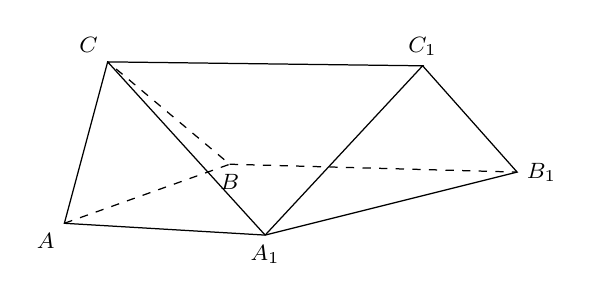
\begin{tikzpicture}[font=\footnotesize, line width=0.45pt]
  \coordinate (A) at (0,0);
  \coordinate (C) at (0.55,2.05);
  \coordinate (B) at (2.10,0.75);
  \coordinate (A1) at (2.55,-0.15);
  \coordinate (C1) at (4.55,2.00);
  \coordinate (B1) at (5.75,0.65);
  \draw (A)--(C)--(C1)--(A1)--cycle;
  \draw (C1)--(B1)--(A1);
  \draw (C)--(A1);
  \draw[dashed] (A)--(B)--(C) (B)--(B1);
  \node[below left] at (A) {$A$};
  \node[above left] at (C) {$C$};
  \node[below] at (B) {$B$};
  \node[below] at (A1) {$A_1$};
  \node[above] at (C1) {$C_1$};
  \node[right] at (B1) {$B_1$};
\end{tikzpicture}
\end{center}
\nopagebreak[4]
(1) 证明：$AB\perp A_1C$；

(2) 若 $AB=CB=2$，$A_1C=\sqrt6$，求三棱柱 $ABC-A_1B_1C_1$ 的体积。

\Needspace{4\baselineskip}
\textbf{解析}

\gksubpart{(1) 证明垂直}

\Needspace{5\baselineskip}
令 $\boldsymbol b=\overrightarrow{AB}$，$\boldsymbol c=\overrightarrow{AC}$，$\boldsymbol u=\overrightarrow{AA_1}$。由 $CA=CB$ 得 $\boldsymbol b\cdot\boldsymbol c=|\boldsymbol b|^2/2$；又因 $AB=AA_1$、$\angle BAA_1=60^\circ$，有 $\boldsymbol b\cdot\boldsymbol u=|\boldsymbol b|^2/2$。于是

\nopagebreak[4]
\[
\boldsymbol b\cdot\overrightarrow{A_1C}
=\boldsymbol b\cdot(\boldsymbol c-\boldsymbol u)=0,
\]

故 $AB\perp A_1C$。

\gksubpart{(2) 求体积}

$\triangle ABC$ 为边长 $2$ 的正三角形。已知 $|\boldsymbol b|=|\boldsymbol c|=|\boldsymbol u|=2$，并有 $\boldsymbol b\cdot\boldsymbol c=2$、$\boldsymbol b\cdot\boldsymbol u=2$、$\boldsymbol c\cdot\boldsymbol u=1$。其 Gram 行列式为 $36$，故 $|[\boldsymbol b,\boldsymbol c,\boldsymbol u]|=6$；三棱柱体积为其一半，即 $3$。

\gkanswer{答案（1）：见解析版}

\gkanswer{答案（2）：$3$}

\end{answer}
\begin{answer}
\gksolhead{20}{}

\textbf{题目}：

已知函数 $f(x)=e^x(ax+b)-x^2-4x$，曲线 $y=f(x)$ 在点 $(0,f(0))$ 处的切线方程为 $y=4x+4$。

(1) 求 $a,b$ 的值；

(2) 讨论 $f(x)$ 的单调性，并求 $f(x)$ 的极大值。

\Needspace{4\baselineskip}
\textbf{解析}

\gksubpart{(1) 求参数}

\Needspace{5\baselineskip}
切线经过 $(0,f(0))$ 且截距为 $4$，故 $b=4$。又

\nopagebreak[4]
\[
f'(0)=a+b-4=4,
\]

所以 $a=4$。

\gksubpart{(2) 单调性与极大值}

\nopagebreak[4]
\[
f'(x)=4e^x(x+2)-2x-4=2(x+2)(2e^x-1).
\]

临界点为 $-2,-\ln2$。符号表给出函数在 $(-\infty,-2)$、$(-\ln2,+\infty)$ 上递增，在 $(-2,-\ln2)$ 上递减；在 $x=-2$ 取得极大值 $4-4/e^2$。

\gkanswer{答案（1）：$a=4,\ b=4$}

\gkanswer{答案（2）：递增区间为 $(-\infty,-2)$、$(-\ln2,+\infty)$，递减区间为 $(-2,-\ln2)$；极大值为 $4-\dfrac4{e^2}$。}

\end{answer}
\begin{answer}
\gksolhead{21}{}

\textbf{题目}：

已知圆 $M:(x+1)^2+y^2=1$，圆 $N:(x-1)^2+y^2=9$，动圆 $P$ 与圆 $M$ 外切并与圆 $N$ 内切，圆心 $P$ 的轨迹为曲线 $C$。

(1) 求 $C$ 的方程；

(2) $l$ 是与圆 $P$、圆 $M$ 都相切的一条直线，$l$ 与曲线 $C$ 交于 $A,B$ 两点，当圆 $P$ 的半径最长时，求 $|AB|$。

\Needspace{4\baselineskip}
\textbf{解析}

\gksubpart{(1) 求轨迹方程}

设动圆半径为 $r$，则 $PM=r+1$、$PN=3-r$，相加得 $PM+PN=4$。两定点为 $(-1,0),(1,0)$，故轨迹为长半轴 $2$、短半轴 $\sqrt3$ 的椭圆：$x^2/4+y^2/3=1$。

\gksubpart{(2) 求弦长}

$PM$ 的最大值为 $3$，此时 $P=(2,0)$、$r=2$。两圆在 $(0,0)$ 外切，共切线为 $x=0$；它与椭圆交于 $(0,\pm\sqrt3)$，故弦长为 $2\sqrt3$。

\gkanswer{答案（1）：$\dfrac{x^2}{4}+\dfrac{y^2}{3}=1$}

\gkanswer{答案（2）：$2\sqrt3$}

\end{answer}
\begin{answer}
\gksolhead{22}{}

\textbf{题目}：

如图，直线 $AB$ 为圆的切线，切点为 $B$，点 $C$ 在圆上，$\angle ABC$ 的角平分线 $BE$ 交圆于点 $E$，$DB\perp BE$ 交圆于 $D$。
\nopagebreak[4]
\begin{center}% 2013 全国卷Ⅰ文科第 22 题：圆、切线、角平分线及弦。
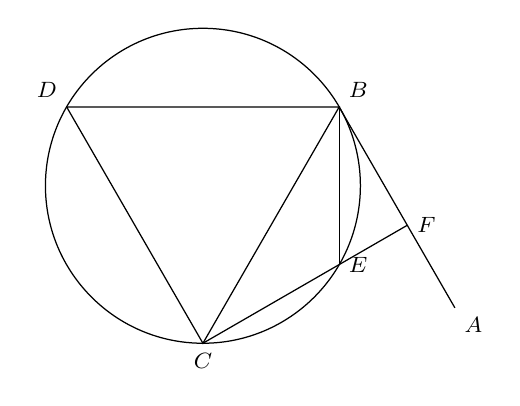
\begin{tikzpicture}[font=\footnotesize, line width=0.45pt]
  \coordinate (O) at (0,0);
  \coordinate (B) at (1.73,1.00);
  \coordinate (D) at (-1.73,1.00);
  \coordinate (C) at (0,-2.00);
  \coordinate (E) at (1.73,-1.00);
  \coordinate (F) at (2.598,-0.50);
  \coordinate (A) at (3.20,-1.55);
  \draw (O) circle (2);
  \draw (D)--(B)--(C)--(D);
  \draw (B)--(E);
  \draw (C)--(F);
  \draw (B)--(A);
  \node[above right] at (B) {$B$};
  \node[above left] at (D) {$D$};
  \node[below] at (C) {$C$};
  \node[right] at (E) {$E$};
  \node[right] at (F) {$F$};
  \node[below right] at (A) {$A$};
\end{tikzpicture}
\end{center}
\nopagebreak[4]
(1) 证明：$DB=DC$；

(2) 设圆的半径为 $1$，$BC=\sqrt3$，延长 $CE$ 交 $AB$ 于点 $F$，求 $\triangle BCF$ 外接圆的半径。

\Needspace{4\baselineskip}
\textbf{解析}

\gksubpart{(1) 证明等长}

\Needspace{5\baselineskip}
令 $\alpha=\angle EBC=\tfrac12\angle ABC$。由 $DB\perp BE$，有 $\angle DBC=90^\circ-\alpha$。又由切线弦定理，切线 $AB$ 与弦 $BC$ 所成的角等于圆周角 $\angle BDC$，故 $\angle BDC=\angle ABC=2\alpha$。在 $\triangle DBC$ 中，

\nopagebreak[4]
\[
\angle BCD=180^\circ-(90^\circ-\alpha)-2\alpha=90^\circ-\alpha=\angle DBC,
\]

所以 $DB=DC$。

\gksubpart{(2) 求外接圆半径}

\Needspace{5\baselineskip}
$BC=\sqrt3$、圆半径为 $1$，故所对圆心角为 $120^\circ$。取圆心角坐标，可得 $\triangle DBC$ 为边长 $\sqrt3$ 的正三角形，且 $BE$ 垂直于其对应方向。由相似或坐标计算得到

\nopagebreak[4]
\[
BC=\sqrt3,\qquad CF=\frac32,\qquad BF=\frac{\sqrt3}{2},\qquad
S_{\triangle BCF}=\frac12\cdot CF\cdot BF=\frac{3\sqrt3}{8}.
\]

并且 $BF^2+CF^2=BC^2$，故 $\angle BFC=90^\circ$，外接圆半径为斜边的一半，即 $\dfrac{\sqrt3}{2}$。

\gkanswer{答案（1）：见解析版}

\gkanswer{答案（2）：$\dfrac{\sqrt3}{2}$}

\end{answer}
\begin{answer}
\gksolhead{23}{}

\textbf{题目}：

\Needspace{5\baselineskip}
已知曲线 $C_1$ 的参数方程为

\nopagebreak[4]
\[
\begin{cases}
x=4+5\cos t,\\
y=5+5\sin t,
\end{cases}\qquad (t\text{ \text{为参数}}),
\]

以坐标原点为极点，$x$ 轴的正半轴为极轴建立极坐标系，曲线 $C_2$ 的极坐标方程为 $\rho=2\sin\theta$。

(1) 把 $C_1$ 的参数方程化为极坐标方程；

(2) 求 $C_1$ 与 $C_2$ 交点的极坐标（$\rho\geqslant0,\ 0\leqslant\theta<2\pi$）。

\Needspace{4\baselineskip}
\textbf{解析}

\gksubpart{(1) 化为极坐标方程}

\Needspace{5\baselineskip}
消去参数得 $(x-4)^2+(y-5)^2=25$。代入 $x=\rho\cos\theta,y=\rho\sin\theta$，整理为

\nopagebreak[4]
\[
\rho^2-8\rho\cos\theta-10\rho\sin\theta+16=0.
\]

\gksubpart{(2) 求交点}

把 $\rho=2\sin\theta$ 代入上式，化为 $\cos\theta(\cos\theta-\sin\theta)=0$。在给定的 $\rho\geqslant0$ 范围内，得到 $\theta=\pi/4,\pi/2$，相应极坐标为 $\left(\sqrt2,\pi/4\right)$、$\left(2,\pi/2\right)$。

\gkanswer{答案（1）：$\rho^2-8\rho\cos\theta-10\rho\sin\theta+16=0$}

\gkanswer{答案（2）：$\left(\sqrt2,\dfrac\pi4\right)$、$\left(2,\dfrac\pi2\right)$}

\end{answer}
\begin{answer}
\gksolhead{24}{}

\textbf{题目}：

已知函数 $f(x)=|2x-1|+|2x+a|$，$g(x)=x+3$。

(1) 当 $a=-2$ 时，求不等式 $f(x)<g(x)$ 的解集；

(2) 设 $a>-1$，且当 $x\in\left[-\dfrac a2,\dfrac12\right]$ 时，$f(x)\leqslant g(x)$，求 $a$ 的取值范围。

\Needspace{4\baselineskip}
\textbf{解析}

\gksubpart{(1) 解绝对值不等式}

令 $a=-2$，按分点 $1/2,1$ 分段化简。三区间分别给出 $x>0$、恒成立、$x<2$，合并为 $(0,2)$。

\gksubpart{(2) 求参数范围}

因 $a>-1$ 且 $x\in[-a/2,1/2]$，此区间内 $2x+a\geqslant0$、$2x-1\leqslant0$，所以 $f(x)=1+a$。要对全区间成立，只须在最小的 $x=-a/2$ 处满足 $1+a\leqslant3-a/2$，即 $a\leqslant4/3$。结合前提得到 $-1<a\leqslant4/3$。

\gkanswer{答案（1）：$(0,2)$}

\gkanswer{答案（2）：$\left(-1,\dfrac43\right]$}

\end{answer}